% =====================================
% EXERCICES : POLYNOMES DU SECOND DEGRE
% Niveau : 1ere Specialite
% =====================================

% Section I : Questions flash
\section{Questions flash}

% Resolution d'equation
\begin{EXO}{Résolution d'équation factorisée}{}
Soit $f$ une fonction définie sur $\R$ par $f(x) = 5(x+1)(x-6)$. 

\tcbitempoint{1} Résoudre l'équation $f(x)=0$.

\begin{crep}
Un produit est nul si et seulement si l'un de ses facteurs est nul.

\begin{tcbenumerate}[3]
\tcbitem $5 = 0$ impossible
\tcbitem $x+1 = 0 \Leftrightarrow x = -1$
\tcbitem $x-6 = 0 \Leftrightarrow x = 6$
\end{tcbenumerate}
$S = \{-1 ; 6\}$
\end{crep}

\exocorrection

On a $f(x) = 5(x+1)(x-6) = 0$.

Un produit est nul si et seulement si l'un de ses facteurs est nul.

\begin{tcbenumerate}[3]
\tcbitem $5 = 0$ impossible
\tcbitem $x+1 = 0 \Leftrightarrow x = -1$
\tcbitem $x-6 = 0 \Leftrightarrow x = 6$
\end{tcbenumerate}

Donc $S = \{-1 ; 6\}$.
\end{EXO}

% Tableau de signe
\begin{EXO}{Tableau de signes avec forme canonique}{}
Soit $f$ une fonction définie sur $\R$ par $f(x) = -2(x-5)^2+13$. 

\tcbitempoint{3} Dresser le tableau de signes de $f$.

\begin{crep}
Racines : $f(x) = 0 \Rightarrow (x-5)^2 = \dfrac{13}{2}$\hfill D'où $x = 5 \pm \sqrt{\dfrac{13}{2}}$\hfill\phantom{a}\\\\
\begin{center}
\begin{tikzpicture}
\tkzTabInit{$x$/1,$f(x)$/1}
{$-\infty$,$5-\sqrt{\frac{13}{2}}$,$5+\sqrt{\frac{13}{2}}$,$+\infty$}
\tkzTabLine{,-,z,+,z,-}
\end{tikzpicture}
\end{center}
\end{crep}

\exocorrection

$f(x) = -2(x-5)^2+13$ est sous forme canonique avec $a = -2 < 0$.

Pour trouver les racines, résolvons $f(x) = 0$ :

$-2(x-5)^2+13 = 0 \Rightarrow (x-5)^2 = \dfrac{13}{2}$

$x-5 = \pm\sqrt{\dfrac{13}{2}} \Rightarrow x = 5 \pm \sqrt{\dfrac{13}{2}}$

Comme $a = -2 < 0$, la parabole est tournée vers le bas.

$f(x) > 0$ entre les racines et $f(x) < 0$ à l'extérieur.
\end{EXO}

% Forme factorisee
\begin{EXO}{Forme factorisée à partir des racines}{}
Soit $f$ la fonction définie sur $\R$ par $f(x)=4x^2-20x-56$. On admet que les racines de $f$ sont $7$ et $-2$. \tcbitempoint{2} Déterminer la forme factorisée de $f$.

\begin{crep}
$f(x) = 4(x-7)(x+2)$
\end{crep}

\exocorrection

Les racines de $f$ sont $x_1 = 7$ et $x_2 = -2$.

La forme factorisée s'écrit $f(x) = a(x-x_1)(x-x_2)$ avec $a$ le coefficient dominant.

Dans la forme développée $f(x) = 4x^2-20x-56$, on lit $a = 4$.

Donc $f(x) = 4(x-7)(x-(-2)) = 4(x-7)(x+2)$.

\textbf{Vérification :} $4(x-7)(x+2) = 4(x^2+2x-7x-14) = 4(x^2-5x-14) = 4x^2-20x-56$ \checkmark
\end{EXO}

% Inequation
\begin{EXO}{Résolution d'inéquation avec forme factorisée}{}
Soit $f$ une fonction définie sur $\R$ par $f(x) = 5(x-2)(x-9)$. 

\tcbitempoint{3} Résoudre l'inéquation $f(x)\geqslant0$.

\begin{crep}
Tableau de signe avec racines $x_1 = 2$ et $x_2 = 9$ :\hfill D'où $S = \CrochetD-\infty;2\CrochetD \cup \CrochetG9;+\infty\CrochetG$\\\\\\\\

\vspace{0.2cm}\begin{center}\begin{tikzpicture}
\tkzTabInit[espcl=2,lgt=1.5]{$x$/0.8,$5$/0.8,$x-2$/0.8,$x-9$/0.8,$f(x)$/0.8}
{$-\infty$,$2$,$9$,$+\infty$}
\tkzTabLine{,+,t,+,t,+,}
\tkzTabLine{,-,z,+,t,+,}
\tkzTabLine{,-,t,-,z,+,}
\tkzTabLine{,+,z,-,z,+,}
\end{tikzpicture}
\end{center}

\end{crep}

\exocorrection

$f(x) = 5(x-2)(x-9) \geqslant 0$

Racines de $f$ : $x_1 = 2$ et $x_2 = 9$.

Coefficient dominant $a = 5 > 0$, donc la parabole est tournée vers le haut.

$f(x) \geqslant 0$ à l'extérieur des racines et $f(x) \leqslant 0$ entre les racines.

Donc $S = \CrochetD-\infty;2\CrochetD \cup \CrochetG9;+\infty\CrochetG$.
\end{EXO}

% Section II : Fonction polynome de degre 2
\section{Fonction polynome de degre 2}

% Reconnaissance degre 2
\begin{EXO}{Reconnaissance de fonctions du second degré}{}
\tcbitempoint{3} Pour chaque fonction ci-dessous, déterminer si c'est une fonction polynôme de degré 2.
\begin{tcbenumerate}[3]
\tcbitem $f(x) = x^2+2x-\sqrt{2}$

\begin{crep}
Oui, $a=1$, $b=2$, $c=-\sqrt{2}$
\end{crep}

\tcbitem $g(x)= x^2+\dfrac{1}{x} -1$

\begin{crep}
Non, présence de $\dfrac{1}{x}$
\end{crep}

\tcbitem $h(x)=3x^2-3x-2x^2+2x-x^2-x+5$

\begin{crep}
Non, degré 0 après réduction
\end{crep}
\end{tcbenumerate}

\exocorrection

\begin{tcbenumerate}[3]
\tcbitem $f(x) = x^2+2x-\sqrt{2}$ est de la forme $ax^2+bx+c$ avec $a=1 \neq 0$, $b=2$, $c=-\sqrt{2}$.

Donc $f$ est une fonction polynôme de degré 2.

\tcbitem $g(x)= x^2+\dfrac{1}{x} -1 = x^2+x^{-1}-1$

La présence du terme $x^{-1}$ (exposant négatif) fait que $g$ n'est pas une fonction polynôme.

\tcbitem $h(x)=3x^2-3x-2x^2+2x-x^2-x+5$

Réduisons : $h(x) = (3-2-1)x^2 + (-3+2-1)x + 5 = 0x^2 - 2x + 5 = -2x + 5$

$h$ est une fonction affine (degré 1), pas une fonction polynôme de degré 2.
\end{tcbenumerate}
\end{EXO}

% Coefficients
\begin{EXO}{Identification des coefficients}{}
\tcbitempoint{6} Parmi les fonctions ci-dessous, indiquer les fonctions polynômes de degré $2$, en précisant ses coefficients.
\begin{tcbenumerate}[3]
\tcbitem $f(x) = (x+3)^2$

\begin{crep}
$f(x) = x^2+6x+9$ donc oui, $a=1$, $b=6$, $c=9$
\end{crep}

\tcbitem $g(x)= (x+3)(x-3)$

\begin{crep}
$g(x) = x^2-9$ donc oui, $a=1$, $b=0$, $c=-9$
\end{crep}

\tcbitem $h(x)= (x+1)^2-(x-1)^2$

\begin{crep}
$h(x) = 4x$ donc non, degré 1
\end{crep}
\end{tcbenumerate}

\exocorrection

\begin{tcbenumerate}[3]
\tcbitem $f(x) = (x+3)^2 = x^2+6x+9$

C'est une fonction polynôme de degré 2 avec $a=1$, $b=6$, $c=9$.

\tcbitem $g(x)= (x+3)(x-3) = x^2-9$

C'est une fonction polynôme de degré 2 avec $a=1$, $b=0$, $c=-9$.

\tcbitem $h(x)= (x+1)^2-(x-1)^2$

Développons : $(x+1)^2 = x^2+2x+1$ et $(x-1)^2 = x^2-2x+1$

Donc $h(x) = (x^2+2x+1)-(x^2-2x+1) = x^2+2x+1-x^2+2x-1 = 4x$

$h$ est une fonction affine (degré 1), pas une fonction polynôme de degré 2.
\end{tcbenumerate}
\end{EXO}

% Developpement
\begin{EXO}{Développement et identification}{}
Soit $f$ la fonction définie sur $\R$ par $ f(x) = 2(x+2)^2 - 3(x+1)$.
\begin{tcbenumerate}[2]
\tcbitem \tcbitempoint{2} Développer $f(x)$.

\begin{crep}
$f(x) = 2(x^2+4x+4) - 3x - 3 $

$\phantom{f(x)}= 2x^2+8x+8-3x-3 $

$\phantom{f(x)}= 2x^2+5x+5$
\end{crep}

\tcbitem \tcbitempoint{1} En déduire que $f$ est une fonction polynôme de degré $2$ et déterminer ses coefficients.

\begin{crep}
$f(x) = 2x^2+5x+5$ donc $a=2$, $b=5$, $c=5$

Comme $a=2 \neq 0$, $f$ est bien de degré 2.
\end{crep}
\end{tcbenumerate}

\exocorrection

\begin{tcbenumerate}[2]
\tcbitem Développement :

$f(x) = 2(x+2)^2 - 3(x+1)$

$= 2(x^2+4x+4) - 3x - 3$

$= 2x^2+8x+8-3x-3$

$= 2x^2+5x+5$

\tcbitem $f(x) = 2x^2+5x+5$ est de la forme $ax^2+bx+c$ avec :

$a = 2 \neq 0$, $b = 5$, $c = 5$

Donc $f$ est bien une fonction polynôme de degré 2.
\end{tcbenumerate}
\end{EXO}

% Section III : Differentes formes d'un polynome de degre 2
\section{Differentes formes d'un polynome de degre 2}

% Forme canonique simple
\begin{EXO}{Forme canonique guidée}{}
Soit $f$ la fonction définie sur $\R$ par $ f(x) = x^2+4x+5$.
\begin{tcbenumerate}[2]
\tcbitem \tcbitempoint{1} Compléter l'égalité ci-contre avec des réels : 
\begin{center}
$x^2+4x+\repsim{4} = (x+\repsim{2})^2$
\end{center}

\tcbitem \tcbitempoint{2} En déduire la forme canonique de $f$.

\begin{crep}
$f(x) = (x+2)^2 + 1$
\end{crep}
\end{tcbenumerate}

\exocorrection

\begin{tcbenumerate}[2]
\tcbitem Pour compléter $(x+\dots)^2$, on cherche $a$ tel que $(x+a)^2 = x^2+2ax+a^2$.

On veut $2ax = 4x$, donc $2a = 4$, donc $a = 2$.

Alors $(x+2)^2 = x^2+4x+4$.

Donc $x^2+4x+4 = (x+2)^2$.

\tcbitem On a $f(x) = x^2+4x+5 = x^2+4x+4+1 = (x+2)^2+1$.

La forme canonique est $f(x) = (x+2)^2 + 1$.
\end{tcbenumerate}
\end{EXO}
\newpage
% Forme canonique guidee
\begin{EXO}{Forme canonique par développement inverse}{}
Soit $f$ la fonction définie sur $\R$ par $ f(x) = -3x^2+24x-41$.
\begin{tcbenumerate}[2]
\tcbitem \tcbitempoint{2} \acc{Développer} l'expression $-3(x-4)^2+7$.

\begin{crep}
$-3(x-4)^2+7 $

$= -3(x^2-8x+16)+7 $

$= -3x^2+24x-48+7 $

$= -3x^2+24x-41$
\end{crep}

\tcbitem \tcbitempoint{1} En déduire la forme canonique de $f$.

\begin{crep}
$f(x) = -3(x-4)^2+7$
\end{crep}
\end{tcbenumerate}

\exocorrection

\begin{tcbenumerate}[2]
\tcbitem Développement de $-3(x-4)^2+7$ :

$-3(x-4)^2+7 = -3(x^2-8x+16)+7$

$= -3x^2+24x-48+7$

$= -3x^2+24x-41$

\tcbitem On constate que $-3(x-4)^2+7 = -3x^2+24x-41 = f(x)$.

Donc la forme canonique de $f$ est : $f(x) = -3(x-4)^2+7$.
\end{tcbenumerate}
\end{EXO}

% Forme canonique entrainement
\begin{EXO}{Forme canonique - Entraînement}{}
\tcbitempoint{4} Déterminer la forme canonique des fonctions suivantes (utiliser un brouillon). 
\begin{tcbenumerate}[2]
\tcbitem $f(x) = x^2-6x+5$
\begin{crep}
$f(x) = ( x - 3 )^2 - 4$
\end{crep}
\tcbitem $f(x) = x^2+5x+4$
\begin{crep}
$f(x) = ( x - \dfrac{5}{2} )^2 - \dfrac{9}{4}$ 
\end{crep}
\end{tcbenumerate}

\exocorrection

D'après le cours : 
L'écriture $a(x-\alpha)^{2} +\beta$ est la\voc{forme canonique} de la fonction $f:x\mapsto ax^{2} + bx + c$.
    
    \begin{tcbenumerate}[1]
        \tcbitem[halign=center] $\alpha = -\dfrac{b}{2a}$
        \tcbitem[halign=center] $\beta = -\dfrac{b^2-4ac}{4a}$
    \end{tcbenumerate}
    \begin{tcbenumerate}[2]
\tcbitem[boxrule=0.4pt,colframe=black,halign=left] $f(x) = x^2-6x+5$
\begin{tcbenumerate}[2][1][alph]
        \tcbitem[halign=center] $\alpha = -\dfrac{-6}{2\times 1} = 3$
        \tcbitem[halign=center] $\beta = -\dfrac{6^2-4\times 1 \times 5}{4\times 1}$
        
        $\phantom{\beta}= -\dfrac{36-20}{4} = -4$
    \end{tcbenumerate}
Ainsi $f(x) = ( x - 3 )^2 - 4$

\tcbitem[boxrule=0.4pt,colframe=black,halign=left] $f(x) = x^2+5x+4$
    \begin{tcbenumerate}[2][1][alph]
        \tcbitem[halign=center] $\alpha = -\dfrac{5}{2}$
        \tcbitem[halign=center] $\beta = -\dfrac{5^2-4\times 1 \times 4}{4\times 1}$
        
        $\phantom{\beta}= -\dfrac{25-16}{4} = -\dfrac{9}{4}$
    \end{tcbenumerate}
$f(x) = ( x - \dfrac{5}{2} )^2 - \dfrac{9}{4}$ 

\end{tcbenumerate}
\end{EXO}

% Forme canonique factorisation
\begin{EXO}{Forme canonique par factorisation}{}
Soit $f$ la fonction définie sur $\R$ par $ f(x) = 2x^2+4x+8$.

\tcbitempoint{2} Déterminer la forme canonique de $f$.
\begin{crep}
$f(x) = 2(x+1)^2 + 6$
\end{crep}

\exocorrection

D'après le cours : 
L'écriture $a(x-\alpha)^{2} +\beta$ est la\voc{forme canonique} de la fonction $f:x\mapsto ax^{2} + bx + c$.

Pour $f(x) = 2x^2+4x+8$, on a $a=2$, $b=4$, $c=8$.

\begin{tcbenumerate}[2][1][alph]
    \tcbitem[halign=center] $\alpha = -\dfrac{b}{2a} = -\dfrac{4}{2 \times 2} = -1$
    \tcbitem[halign=center] $\beta = -\dfrac{b^2-4ac}{4a} = -\dfrac{4^2-4 \times 2 \times 8}{4 \times 2}$
    
    $\phantom{\beta}= -\dfrac{16-64}{8} = -\dfrac{-48}{8} = 6$
\end{tcbenumerate}

En remplaçant $a$, $\alpha$ et $\beta$  dans l'expression de la forme canonique, on obtient: 
$$f(x) = 2(x+1)^2 + 6$$
\end{EXO}

% Forme canonique avance
\begin{EXO}{Forme canonique - Niveau avancé}{}
\tcbitempoint{6} Déterminer la forme canonique des fonctions suivantes (utiliser un brouillon). 
\begin{tcbenumerate}[2]
\tcbitem $f(x) = 3x^2+9x+5$
\begin{crep}
$f(x) = 3(x + \dfrac{3}{2})^2 - \dfrac{7}{4}$
\end{crep}
\tcbitem $f(x) = -2x^2+2x+2$
\begin{crep}
$f(x) = -2(x - \dfrac{1}{2})^2 + \dfrac{5}{2}$
\end{crep}
\end{tcbenumerate}

\exocorrection

D'après le cours : 
L'écriture $a(x-\alpha)^{2} +\beta$ est la\voc{forme canonique} de la fonction $f:x\mapsto ax^{2} + bx + c$.
    
    \begin{tcbenumerate}[2]
        \tcbitem[halign=center] $\alpha = -\dfrac{b}{2a}$
        \tcbitem[halign=center] $\beta = -\dfrac{b^2-4ac}{4a}$
    \end{tcbenumerate}
    
\begin{tcbenumerate}[1]
\tcbitem[boxrule=0.4pt,colframe=black,halign=left] $f(x) = 3x^2+9x+5$

Pour cette fonction, on a $a=3$, $b=9$, $c=5$.

\begin{tcbenumerate}[2][1][alph]
    \tcbitem[halign=center] $\alpha = -\dfrac{b}{2a} = -\dfrac{9}{2 \times 3} = -\dfrac{9}{6} = -\dfrac{3}{2}$
    \tcbitem[halign=center] $\beta = -\dfrac{b^2-4ac}{4a} = -\dfrac{9^2-4 \times 3 \times 5}{4 \times 3}$
    
    $\phantom{\beta}= -\dfrac{81-60}{12} = -\dfrac{21}{12} = -\dfrac{7}{4}$
\end{tcbenumerate}

Ainsi $f(x) = 3(x - (-\dfrac{3}{2}))^2 + (-\dfrac{7}{4}) = 3(x + \dfrac{3}{2})^2 - \dfrac{7}{4}$

\tcbitem[boxrule=0.4pt,colframe=black,halign=left] $f(x) = -2x^2+2x+2$

Pour cette fonction, on a $a=-2$, $b=2$, $c=2$.

\begin{tcbenumerate}[2][1][alph]
    \tcbitem[halign=center] $\alpha = -\dfrac{b}{2a} = -\dfrac{2}{2 \times (-2)} = -\dfrac{2}{-4} = \dfrac{1}{2}$
    \tcbitem[halign=center] $\beta = -\dfrac{b^2-4ac}{4a} = -\dfrac{2^2-4 \times (-2) \times 2}{4 \times (-2)}$
    
    $\phantom{\beta}= -\dfrac{4-(-16)}{-8} = -\dfrac{4+16}{-8} = -\dfrac{20}{-8} = \dfrac{5}{2}$
\end{tcbenumerate}

Ainsi $f(x) = -2(x - \dfrac{1}{2})^2 + \dfrac{5}{2}$
\end{tcbenumerate}
\end{EXO}

% Trois formes
\begin{EXO}{Trois formes d'une fonction du second degré}{}
Soit $f$ la fonction définie sur $\R$ par $ f(x) = 2x^2+4x-16$.
\begin{tcbenumerate}[2]
\tcbitem \tcbitempoint{2} Montrer que pour tout réel $x$, 
\vspace{-0.3cm}\begin{center}$f(x) = 2(x+4)(x-2)$\end{center}
\begin{crep}
$2(x+4)(x-2) $

$= 2(x^2-2x+4x-8 ) $

$= 2x^2+ 4x -16 $

$= f(x)$

\end{crep}

\tcbitem \tcbitempoint{2} Montrer que pour tout réel $x$, 
\vspace{-0.3cm}\begin{center}$f(x) = 2(x+1)^2-18$\end{center}
\begin{crep}
$2(x+1)^2-18 $

$= 2(x^2+2x+1)-18 $

$= 2x^2+4x+2-18 $

$= 2x^2+4x-16= f(x)$ 
\end{crep}
\end{tcbenumerate}
\begin{tcbenumerate}[2][3]
\tcbitem[colframe=black,boxrule=0.4pt,raster multicolumn=2] Choisir la forme la plus adaptée pour répondre aux questions suivantes.
\begin{tcbenumerate}[2][1][alph]
\tcbitem \tcbitempoint{3} Dresser le tableau de variations de $f$
\setrdcrep{seyes=false,correction color=black,correction font=\normalsize}
\begin{crep}[colback=white,colframe=white]%[extra lines=2]
Forme canonique : $f(x) = 2(x+1)^2-18$\\\\

\begin{tikzpicture}
\tkzTabInit{$x$/1,$f$/1.8}
{$-\infty$,$-1$,$+\infty$}
\tkzTabVar{+/$+\infty$,-/$-18$,+/$+\infty$}
\end{tikzpicture}
\end{crep}

\tcbitem \tcbitempoint{1} Résoudre $f(x)=0$

\begin{crep}
Forme factorisée : 

$f(x) = 2(x+1+3)(x+1-3) $

$\phantom{f(x)}= 2(x+4)(x-2)$

$S = \{-4 ; 2\}$
\end{crep}

\tcbitem \tcbitempoint{2} Résoudre $f(x)=-16$

\begin{crep}
Forme développée : $2x^2+4x-16 = -16$

$2x^2+4x = 0 \Rightarrow x(2x+4) = 0$

$S = \{-2 ; 0\}$
\end{crep}

\tcbitem \tcbitempoint{3} Résoudre $f(x)>0$

\begin{crep}
Forme factorisée avec $f(x) = 2(x+4)(x-2)$

$S = \CrochetD-\infty;-4\CrochetG \cup \CrochetD2;+\infty\CrochetG$
\end{crep}
\end{tcbenumerate}
\end{tcbenumerate}

\exocorrection

\begin{tcbenumerate}[2]
\tcbitem \tcbitempoint{2} Montrer que pour tout réel $x$, 
\vspace{-0.3cm}\begin{center}$f(x) = 2(x+4)(x-2)$\end{center}
\begin{crep}
$2(x+4)(x-2) $

$= 2(x^2-2x+4x-8 ) $

$= 2x^2+ 4x -16 $

$= f(x)$

\end{crep}

\tcbitem \tcbitempoint{2} Montrer que pour tout réel $x$, 
\vspace{-0.3cm}\begin{center}$f(x) = 2(x+1)^2-18$\end{center}
\begin{crep}
$2(x+1)^2-18 $

$= 2(x^2+2x+1)-18 $

$= 2x^2+4x+2-18 $

$= 2x^2+4x-16= f(x)$ 
\end{crep}
\end{tcbenumerate}
\begin{tcbenumerate}[2][3]
\tcbitem[colframe=black,boxrule=0.4pt,raster multicolumn=2] Choisir la forme la plus adaptée pour répondre aux questions suivantes.
\begin{tcbenumerate}[2][1][alph]
\tcbitem \tcbitempoint{3} Dresser le tableau de variations de $f$
\setrdcrep{seyes=false,correction color=black,correction font=\normalsize}
\begin{crep}[colback=white,colframe=white]%[extra lines=2]
Forme canonique : $f(x) = 2(x+1)^2-18$\\\\

\begin{tikzpicture}
\tkzTabInit{$x$/1,$f$/1.8}
{$-\infty$,$-1$,$+\infty$}
\tkzTabVar{+/$+\infty$,-/$-18$,+/$+\infty$}
\end{tikzpicture}
\end{crep}

\tcbitem \tcbitempoint{1} Résoudre $f(x)=0$

\begin{crep}
Forme factorisée : 

$f(x) = 2(x+1+3)(x+1-3) $

$\phantom{f(x)}= 2(x+4)(x-2)$

$S = \{-4 ; 2\}$
\end{crep}

\tcbitem \tcbitempoint{2} Résoudre $f(x)=-16$

\begin{crep}
Forme développée : $2x^2+4x-16 = -16$

$2x^2+4x = 0 \Rightarrow x(2x+4) = 0$

$S = \{-2 ; 0\}$
\end{crep}

\tcbitem \tcbitempoint{3} Résoudre $f(x)>0$

\begin{crep}
Forme factorisée avec $f(x) = 2(x+4)(x-2)$

$S = \CrochetD-\infty;-4\CrochetG \cup \CrochetD2;+\infty\CrochetG$
\end{crep}
\end{tcbenumerate}
\end{tcbenumerate}
\end{EXO}

% Trois formes resolutions
\begin{EXO}{Formes et résolutions d'équations}{}
Soit $f$ la fonction définie sur $\R$ par $ f(x) = (x+2)^2-9$.
\begin{tcbenumerate}[2]
\tcbitem \tcbitempoint{2} Développer et réduire $f(x)$

\begin{crep}
$f(x) = x^2+4x+4-9 $

$= x^2+4x-5$
\end{crep}

\tcbitem \tcbitempoint{2} Factoriser $f(x)$.

\begin{crep}
$f(x) = (x+2)^2-9 $

$= (x+2)^2-3^2 $

$= (x+2-3)(x+2+3) $

$= (x-1)(x+5)$
\end{crep}
\end{tcbenumerate}
\begin{tcbenumerate}[1][3]
\tcbitem[colframe=black,boxrule=0.4pt] Résoudre en utilisant la forme la plus adaptée.
\vspace{-2mm}
\begin{tcbenumerate}[3][1][alph]
\tcbitem \tcbitempoint{3} $f(x)=9$

\begin{crep}
$(x+2)^2-9 = 9 $

$\Rightarrow (x+2)^2 = 18$

$\Rightarrow x+2 = \pm \sqrt{18} = \pm 3\sqrt{2}$

$\Rightarrow x = -2 \pm 3\sqrt{2}$

$S = \{-2 - 3\sqrt{2} ; -2 + 3\sqrt{2}\}$
\end{crep}

\tcbitem \tcbitempoint{1} $f(x)=0$

\begin{crep}
$(x-1)(x+5) = 0$

$S = \{1 ; -5\}$
\end{crep}

\tcbitem \tcbitempoint{2} $f(x)=-5$

\begin{crep}
$x^2+4x-5 = -5$

$\Rightarrow x^2+4x = 0$

$x(x+4) = 0 \Rightarrow S = \{0 ; -4\}$
\end{crep}
\end{tcbenumerate}
\end{tcbenumerate}

\exocorrection

\begin{tcbenumerate}[2]
\tcbitem \tcbitempoint{2} Développer et réduire $f(x)$

\begin{crep}
$f(x) = x^2+4x+4-9 $

$= x^2+4x-5$
\end{crep}

\tcbitem \tcbitempoint{2} Factoriser $f(x)$.

\begin{crep}
$f(x) = (x+2)^2-9 $

$= (x+2)^2-3^2 $

$= (x+2-3)(x+2+3) $

$= (x-1)(x+5)$
\end{crep}
\end{tcbenumerate}
\begin{tcbenumerate}[1][3]
\tcbitem[colframe=black,boxrule=0.4pt] Résoudre en utilisant la forme la plus adaptée.
\vspace{-2mm}
\begin{tcbenumerate}[3][1][alph]
\tcbitem \tcbitempoint{3} $f(x)=9$

\begin{crep}
$(x+2)^2-9 = 9 $

$\Rightarrow (x+2)^2 = 18$

$\Rightarrow x+2 = \pm \sqrt{18} = \pm 3\sqrt{2}$

$\Rightarrow x = -2 \pm 3\sqrt{2}$

$S = \{-2 - 3\sqrt{2} ; -2 + 3\sqrt{2}\}$
\end{crep}

\tcbitem \tcbitempoint{1} $f(x)=0$

\begin{crep}
$(x-1)(x+5) = 0$

$S = \{1 ; -5\}$
\end{crep}

\tcbitem \tcbitempoint{2} $f(x)=-5$

\begin{crep}
$x^2+4x-5 = -5$

$\Rightarrow x^2+4x = 0$

$x(x+4) = 0 \Rightarrow S = \{0 ; -4\}$
\end{crep}
\end{tcbenumerate}
\end{tcbenumerate}
\end{EXO}
\newpage
% Probleme poids
\begin{EXO}{Modélisation d'une évolution de poids}{}
Une personne s'est pesée toutes les semaines pendant un an en 2018. Sa courbe de poids peut être modélisée par une fonction polynôme de degré 2 dont l'expression est $f(x)=0.008x^2-0.4x+75$ où $x$ correspond au temps en semaines à partir du premier janvier 2018 ($x\in \CrochetG0;52\CrochetD$).
\begin{tcbenumerate}[2]
\tcbitem \tcbitempoint{3} Dresser le tableau de variations de la fonction $f$.
\setrdcrep{seyes=false,correction color=black,correction font=\normalsize}
\begin{crep}[colback=white,colframe=white]
Forme canonique : $f(x) = 0{,}008(x-25)^2 + 70$\\\\

\begin{tikzpicture}
\tkzTabInit{$x$/1,$f$/1.8}
{$0$,$25$,$52$}
\tkzTabVar{+/$75$,-/$70$,+/$75{,}632$}
\end{tikzpicture}
\end{crep}

\tcbitem[colframe=black,boxrule=0.4pt] En utilisant cette modélisation, répondre aux questions suivantes.
\begin{tcbenumerate}[2][1][alph]
\tcbitem \tcbitempoint{1} Quel était son poids maximal sur l'année ? Quand a-t-il été atteint ?

\begin{crep}
Poids maximal : $75{,}632$ kg atteint à la semaine $52$
\end{crep}

\tcbitem \tcbitempoint{1} Quel était son poids minimal sur l'année ? Quand a-t-il été atteint ?

\begin{crep}
Poids minimal : $70$ kg atteint à la semaine $25$
\end{crep}
\end{tcbenumerate}
\end{tcbenumerate}

\exocorrection

\begin{tcbenumerate}[2]
\tcbitem Pour dresser le tableau de variations, déterminons la forme canonique :

$f(x) = 0{,}008x^2 - 0{,}4x + 75$

$\alpha = -\dfrac{b}{2a} = -\dfrac{-0{,}4}{2 \times 0{,}008} = \dfrac{0{,}4}{0{,}016} = 25$

$\beta = f(25) = 0{,}008 \times 25^2 - 0{,}4 \times 25 + 75 = 5 - 10 + 75 = 70$

Donc $f(x) = 0{,}008(x-25)^2 + 70$.

Comme $a = 0{,}008 > 0$, la parabole est tournée vers le haut.

Sur $\CrochetG0;52\CrochetD$ : minimum en $x = 25$ avec $f(25) = 70$.

Aux bornes : $f(0) = 75$ et $f(52) = 0{,}008 \times 27^2 + 70 = 5{,}832 + 70 = 75{,}632$

\tcbitem D'après le tableau de variations :
\begin{tcbenumerate}[2]
\tcbitem Le poids maximal est $75{,}632$ kg, atteint à la fin de l'année (semaine 52).
\tcbitem Le poids minimal est $70$ kg, atteint à la semaine 25 (fin juin).
\end{tcbenumerate}
\end{tcbenumerate}
\end{EXO}

% Section IV : Variations et courbe representative
\section{Variations et courbe representative}

% Lecture graphique
\begin{EXO}{Lecture graphique de paraboles}{}
\tcbitempoint{3} Pour chaque fonction représentée ci-dessous, déterminer les coordonnées du sommet, l'axe de symétrie et le signe de $a$.

\begin{MultiColonnes}{4}[boxrule=0.4pt,colframe=black]
\tcbitem[halign=center]
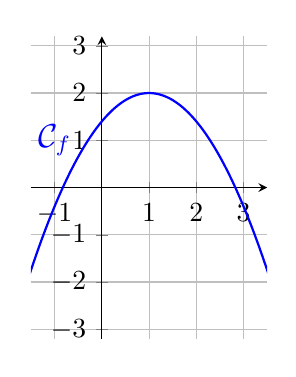
\begin{tikzpicture}
\begin{axis}[
x=1.0cm,y=1.0cm,scale=0.6,
axis lines=middle,
ymajorgrids=true,
xmajorgrids=true,
xmin=-1.5,
xmax=3.5,
ymin=-3.2,
ymax=3.2,
xtick={-1.0,0.0,...,3.0},
ytick={-3.0,-2.0,...,3.0},]
\clip(-1.5,-3.2) rectangle (3.5,3.2);
\addplot[thick,blue, samples=200] {-0.6*(x-1)^2+2};
\begin{scriptsize}
\draw[color=blue] (-1,1) node {\large{$\mathcal{C}_f$}};
\end{scriptsize}
\end{axis}
\end{tikzpicture}

Sommet : \tcfillcrep{$(1;2)$}

Axe : \tcfillcrep{$x=1$}
  
Signe de $a$ : \tcfillcrep{$a<0$}


\tcbitem[halign=center]
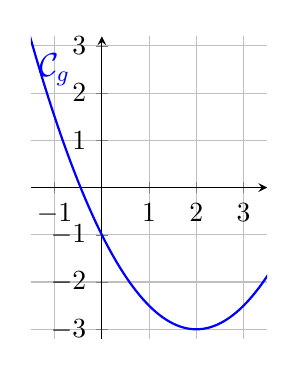
\begin{tikzpicture}
\begin{axis}[
x=1.0cm,y=1.0cm,scale=0.6,
axis lines=middle,
ymajorgrids=true,
xmajorgrids=true,
xmin=-1.5,
xmax=3.5,
ymin=-3.2,
ymax=3.2,
xtick={-1.0,0.0,...,3.0},
ytick={-3.0,-2.0,...,3.0},]
\clip(-1.5,-3.2) rectangle (3.5,3.2);
\addplot[thick,blue, samples=200] {0.5*(x-2)^2-3};
\begin{scriptsize}
\draw[color=blue] (-1,2.5) node {\large{$\mathcal{C}_g$}};
\end{scriptsize}
\end{axis}
\end{tikzpicture}

Sommet : \tcfillcrep{$(2;-3)$}

Axe : \tcfillcrep{$x=2$}
  
Signe de $a$ : \tcfillcrep{$a>0$}


\tcbitem[halign=center]
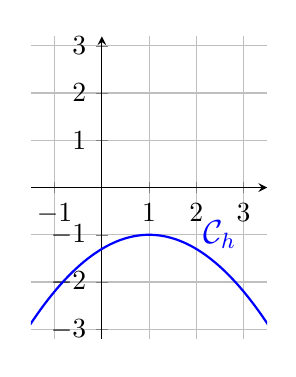
\begin{tikzpicture}
\begin{axis}[
x=1.0cm,y=1.0cm,scale=0.6,
axis lines=middle,
ymajorgrids=true,
xmajorgrids=true,
xmin=-1.5,
xmax=3.5,
ymin=-3.2,
ymax=3.2,
xtick={-1.0,0.0,...,3.0},
ytick={-3.0,-2.0,...,3.0},]
\clip(-1.5,-3.2) rectangle (3.5,3.2);
\addplot[thick,blue, samples=200] {-0.3*(x-1)^2-1};
\begin{scriptsize}
\draw[color=blue] (2.5,-1) node {\large{$\mathcal{C}_h$}};
\end{scriptsize}
\end{axis}
\end{tikzpicture}

Sommet : \tcfillcrep{$(1;-1)$}

Axe : \tcfillcrep{$x=1$}
  
Signe de $a$ : \tcfillcrep{$a<0$}


\tcbitem[halign=center]
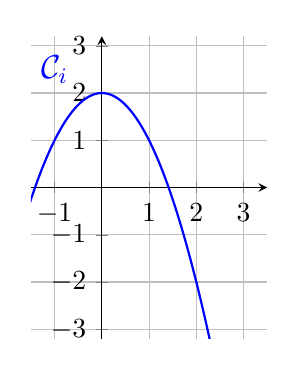
\begin{tikzpicture}
\begin{axis}[
x=1.0cm,y=1.0cm,scale=0.6,
axis lines=middle,
ymajorgrids=true,
xmajorgrids=true,
xmin=-1.5,
xmax=3.5,
ymin=-3.2,
ymax=3.2,
xtick={-1.0,0.0,...,3.0},
ytick={-3.0,-2.0,...,3.0},]
\clip(-1.5,-3.2) rectangle (3.5,3.2);
\addplot[thick,blue, samples=200] {-1*x^2+2};
\begin{scriptsize}
\draw[color=blue] (-1,2.5) node {\large{$\mathcal{C}_i$}};
\end{scriptsize}
\end{axis}
\end{tikzpicture}

Sommet : \tcfillcrep{$(0;2)$}

Axe : \tcfillcrep{$x=0$}
  
Signe de $a$ : \tcfillcrep{$a<0$}

\end{MultiColonnes}

\exocorrection

Pour chaque parabole, je lis graphiquement :

\begin{MultiColonnes}{4}
\tcbitem[halign=center] $\mathcal{C}_f$ : 
\begin{itemize}
\item Sommet au point le plus haut : $(1;2)$
\item Axe de symétrie vertical : $x=1$ 
\item Parabole vers le bas : $a<0$
\end{itemize}

\tcbitem[halign=center] $\mathcal{C}_g$ :
\begin{itemize}
\item Sommet au point le plus bas : $(2;-3)$
\item Axe de symétrie vertical : $x=2$
\item Parabole vers le haut : $a>0$
\end{itemize}

\tcbitem[halign=center] $\mathcal{C}_h$ :
\begin{itemize}
\item Sommet au point le plus haut : $(1;-1)$
\item Axe de symétrie vertical : $x=1$
\item Parabole vers le bas : $a<0$
\end{itemize}

\tcbitem[halign=center] $\mathcal{C}_i$ :
\begin{itemize}
\item Sommet au point le plus haut : $(0;2)$
\item Axe de symétrie vertical : $x=0$
\item Parabole vers le bas : $a<0$
\end{itemize}
\end{MultiColonnes}
\end{EXO}

% Min/max des fonctions  
\begin{EXO}{Minimum et maximum de fonctions}{}
\tcbitempoint{4} Dire pour chaque fonction si elle admet un minimum ou un maximum et en quelle valeur il est atteint.

\begin{tcbenumerate}[4]
\tcbitem $f(x) = 3x^2+4$

\begin{crep}
Minimum en $x=0$,

vaut $f(0)=4$
\end{crep}

\tcbitem $g(x)= -2(x-4)^2+8$

\begin{crep}
Maximum en 

$x=4$, vaut $g(4)=8$
\end{crep}

\tcbitem $h(x)= -2x^2+8x-1$

\begin{crep}
Maximum en 

$x=2$, vaut $h(2)=7$
\end{crep}

\tcbitem $k(x)= 7(x+1)^2-25$

\begin{crep}
Minimum en $x=-1$, 

vaut $k(-1)=-25$
\end{crep}
\end{tcbenumerate}

\exocorrection

\begin{tcbenumerate}[2]
\tcbitem $f(x) = 3x^2+4 = 3(x-0)^2+4$

Forme canonique : $a=3>0$, donc minimum.

Minimum atteint en $x=0$ avec $f(0)=4$.

\tcbitem $g(x)= -2(x-4)^2+8$

Forme canonique : $a=-2<0$, donc maximum.

Maximum atteint en $x=4$ avec $g(4)=8$.

\tcbitem $h(x)= -2x^2+8x-1$

Forme canonique : $\alpha = -\dfrac{8}{2 \times (-2)} = 2$

$\beta = h(2) = -2 \times 4 + 8 \times 2 - 1 = 7$

Donc $h(x) = -2(x-2)^2+7$ avec $a=-2<0$.

Maximum atteint en $x=2$ avec $h(2)=7$.

\tcbitem $k(x)= 7(x+1)^2-25$

Forme canonique : $a=7>0$, donc minimum.

Minimum atteint en $x=-1$ avec $k(-1)=-25$.
\end{tcbenumerate}
\end{EXO}
\newpage
% Variations de fonction
\begin{EXO}{Variations d'une fonction du second degré}{}
Soit $f$ une fonction définie sur $\R$ par $f(x) = x^2+x-2$.

\begin{tcbenumerate}[3]
\tcbitem \tcbitempoint{1} Calculer $f(1)$

\begin{crep}
$f(1) = 1^2 + 1 - 2 = 0$
\end{crep}

\tcbitem[raster multicolumn=2] \tcbitempoint{2} Déterminer la forme canonique de $f$.

\begin{crep}[extra lines=1]
$f(x) = x^2 + x - 2$, on a  $\alpha = -\dfrac{1}{2 \times 1} = -\dfrac{1}{2}$\\[0.6em]
$\beta = f\left(-\dfrac{1}{2}\right)= \left(-\dfrac{1}{2}\right)^2 + \left(-\dfrac{1}{2}\right) - 2 $\\[0.6em]
$= \dfrac{1}{4} - \dfrac{1}{2} - 2 = -\dfrac{9}{4}$\\[0.6em]
Donc $f(x) = \left(x + \dfrac{1}{2}\right)^2 - \dfrac{9}{4}$
\end{crep}

\tcbitem[raster multicolumn=3] \tcbitempoint{3} Dresser le tableau de variations de $f$.
\setrdcrep{seyes=false,correction color=black,correction font=\normalsize}
\begin{crep}[colframe=white, colback=white]


\begin{center}
\begin{tikzpicture}
\tkzTabInit{$x$/1,$f(x)$/1.2}
{$-\infty$,$-\frac{1}{2}$,$+\infty$}
\tkzTabVar{+/$+\infty$,-/$-\frac{9}{4}$,+/$+\infty$}
\end{tikzpicture}
\end{center}
\end{crep}
\end{tcbenumerate}

\exocorrection

\begin{tcbenumerate}[3]
\tcbitem $f(1) = 1^2 + 1 - 2 = 1 + 1 - 2 = 0$

\tcbitem Pour déterminer la forme canonique de $f(x) = x^2 + x - 2$ :

Coefficient dominant $a = 1 > 0$, coefficient de $x$ : $b = 1$.

$\alpha = -\dfrac{b}{2a} = -\dfrac{1}{2 \times 1} = -\dfrac{1}{2}$

$\beta = f\left(-\dfrac{1}{2}\right) = \left(-\dfrac{1}{2}\right)^2 + \left(-\dfrac{1}{2}\right) - 2$

$\beta = \dfrac{1}{4} - \dfrac{1}{2} - 2 = \dfrac{1}{4} - \dfrac{2}{4} - \dfrac{8}{4} = -\dfrac{9}{4}$

Donc la forme canonique est : $f(x) = \left(x + \dfrac{1}{2}\right)^2 - \dfrac{9}{4}$

\tcbitem Puisque $a = 1 > 0$, la parabole est tournée vers le haut.

La fonction admet un minimum en $x = -\dfrac{1}{2}$ avec $f\left(-\dfrac{1}{2}\right) = -\dfrac{9}{4}$.

La fonction est décroissante sur $\CrochetD-\infty ; -\dfrac{1}{2}\CrochetD$ et croissante sur $\CrochetG-\dfrac{1}{2} ; +\infty\CrochetG$.
\end{tcbenumerate}
\end{EXO}

% Forme canonique avec sommet et point
\begin{EXO}{Détermination d'une parabole par son sommet}{}
Soit $f$ une fonction polynôme de degré 2. La courbe représentative de $f$ a pour sommet le point $A(1;3)$ et passe par le point $B(0;5)$. 

\tcbitempoint{3} Déterminer la forme canonique de $f$.

\begin{crep}
La forme canonique est $f(x) = a(x-\alpha)^2 + \beta$ avec sommet $(\alpha;\beta)$.

Ici $\alpha = 1$ et $\beta = 3$, donc $f(x) = a(x-1)^2 + 3$.

La courbe passe par $B(0;5)$ donc $f(0) = 5$

$a(0-1)^2 + 3 = 5$, donc $a \times 1 + 3 = 5$ 

Ainsi, $a = 2$ et $f(x) = 2(x-1)^2 + 3$
\end{crep}

\exocorrection

Puisque $f$ est une fonction polynôme de degré 2, sa forme canonique est :
\begin{center}$f(x) = a(x-\alpha)^2 + \beta$\end{center}

où $(\alpha;\beta)$ sont les coordonnées du sommet.

D'après l'énoncé, le sommet est $A(1;3)$, donc :
- $\alpha = 1$
- $\beta = 3$

La forme canonique devient : $f(x) = a(x-1)^2 + 3$

Il reste à déterminer le coefficient $a$. 

La courbe passe par le point $B(0;5)$, donc $f(0) = 5$ :

$f(0) = a(0-1)^2 + 3 = a \times 1 + 3 = a + 3$

Puisque $f(0) = 5$ :
\begin{center}$a + 3 = 5 \Leftrightarrow a = 2$\end{center}

La forme canonique de $f$ est donc : \begin{center}$f(x) = 2(x-1)^2 + 3$\end{center}
\end{EXO}

% Lecture graphique avec courbe
\begin{EXO}{Forme canonique par lecture graphique}{}
Soit $f$ la fonction dont la représentation graphique est donnée ci-contre. 

\begin{MultiColonnes}{3}
    \tcbitem[raster multicolumn=2] \tcbitempoint{3} Déterminer la forme canonique de $f$.

\begin{crep}
- Sommet : $A(1;2)$ donc $\alpha = 1$ et $\beta = 2$

- Point $B(0;4)$ appartient à la courbe

Forme canonique : $f(x) = a(x-1)^2 + 2$

Puisque $f(0) = 4$, $a(0-1)^2 + 2 = 4$

D'où $a + 2 = 4 \Longrightarrow a = 2$ et $f(x) = 2(x-1)^2 + 2$
\end{crep}

    \tcbitem \begin{tikzpicture}[line cap=round,line join=round,>=triangle 45,x=1.0cm,y=1.0cm,scale=0.8]
\begin{axis}[
x=1.0cm,y=1.0cm,
axis lines=middle,
ymajorgrids=true,
xmajorgrids=true,
xmin=-1.5,
xmax=3.5,
ymin=-0.5,
ymax=5.5,
xtick={-1.0,0.0,...,3.0},
ytick={-0.0,1.0,...,5.0},]
\clip(-1.5,-0.5) rectangle (3.5,5.5);
\addplot[thick,monrose,samples=200] {2*(x-1)^2+2};
\begin{scriptsize}
\draw[color=monrose] (0.24,5) node {$\mathcal{C}_f$};
\draw [fill=black] (1.,2.) circle (3.0pt);
\draw[color=black] (0.9,2.55) node {$A$};
\draw [fill=black] (0.,4.) circle (3.0pt);
\draw[color=black] (0.34,4.43) node {$B$};
\end{scriptsize}
\end{axis}
\end{tikzpicture}
    
\end{MultiColonnes}

\exocorrection

En observant la représentation graphique, je peux identifier :

\textbf{1) Le sommet de la parabole :} 

Le point le plus bas de la courbe est $A(1;2)$, donc :

- $\alpha = 1$ (abscisse du sommet)

- $\beta = 2$ (ordonnée du sommet)

\textbf{2) La forme canonique partielle :}

$f(x) = a(x-\alpha)^2 + \beta = a(x-1)^2 + 2$

\textbf{3) Détermination du coefficient $a$ :}

La courbe passe par le point $B(0;4)$, donc $f(0) = 4$ :

$f(0) = a(0-1)^2 + 2 = a \times 1 + 2 = a + 2$

Puisque $f(0) = 4$ :
\begin{center}$a + 2 = 4 \Leftrightarrow a = 2$\end{center}

\textbf{4) Forme canonique finale :}

\begin{center}$f(x) = 2(x-1)^2 + 2$\end{center}

Vérification : $f(0) = 2(0-1)^2 + 2 = 2 \times 1 + 2 = 4$ ✓
\end{EXO}

% =====================================
% FIN DU DOCUMENT
% =====================================